\documentclass[border = 3mmm]{standalone}
\usepackage{pgfplots}
\usepgfplotslibrary{groupplots}
\pgfplotsset{width=10cm,compat=newest}  % <<height>>

\begin{document}

\begin{tabular}{c}
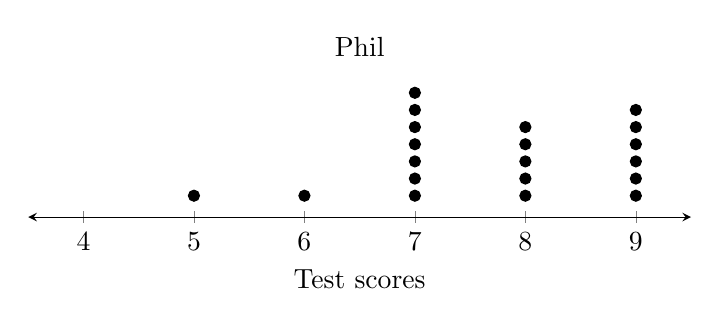
\begin{tikzpicture}
    \begin{axis}[
        height=3.15cm,
        xmin=3.5,
        xmax=9.5,
        % hide y axis,
        axis y line=none,
        axis x line=bottom,
        % set the precision of the x tick labels to be 0, which means no decimals
        % xticklabel style={/pgf/number format/precision=0},
        xtick={4,5,...,9},
        axis x line shift={4pt},
        every outer x axis line/.append style={stealth-stealth},
        title={Phil},
        xlabel={Test scores}]
        \addplot [only marks, black, mark=*, mark size=2pt] coordinates{(5, 1)(6, 1)(7, 1)(7, 2)(7, 3)(7, 4)(7, 5)(7, 6)(7, 7)(8, 1)(8, 2)(8, 3)(8, 4)(8, 5)(9, 1)(9, 2)(9, 3)(9, 4)(9, 5)(9, 6)};
    \end{axis}
\end{tikzpicture}
\\
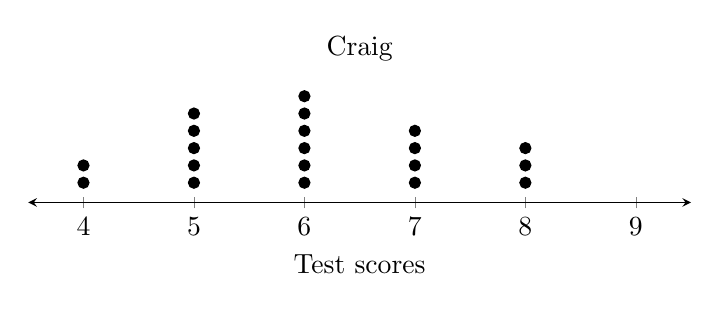
\begin{tikzpicture}
    \begin{axis}[
    height=2.9cm,
    xmin=3.5,
    xmax=9.5,
    % hide y axis,
    axis y line=none,
    axis x line=bottom,
    xtick={4,5,...,9},
    axis x line shift={4pt},
    every outer x axis line/.append style={stealth-stealth},
    mark=*,
    title={Craig},
    xlabel={Test scores}]
    \addplot [only marks] coordinates{(4, 1)(4, 2)(5, 1)(5, 2)(5, 3)(5, 4)(5, 5)(6, 1)(6, 2)(6, 3)(6, 4)(6, 5)(6, 6)(7, 1)(7, 2)(7, 3)(7, 4)(8, 1)(8, 2)(8, 3)};
    \end{axis}
\end{tikzpicture}
\\
\end{tabular}

\end{document}


